\section{8th Sheaf Cobordism'}
Suppose we have a punctured Riemann sphere $M$ and $\Lambda_0^0$, $\Lambda_0^\infty$, $\Lambda_0^{squig}$, a nested regions $U\subset U' \subset M$, and a chart $f : U \rightarrow \R^2$ such that $U'$ maps to $R:=(-2,2)_x \times (-1,1)_z$ under $f$
\begin{itemize}
\item $\Lambda_0^0$ gets mapped to $\{(x,z)\in R \mid z=\Psi(z_{lo} = 0,z_{hi}=1)(x)\}$, co-oriented upward.

\item $\Lambda_0^\infty$ gets mapped to $\{(x,z)\in R \mid z=\tau(\frac{x+1}{2})-\frac{1}{2}\}\cup \{(x,z)\in R \mid z=-\tau(\frac{x+1}{2})+\frac{1}{2}\}$, co-oriented downward.

\item $\Lambda_0^{squig}$ gets mapped to $\{(x,z)\in R \mid x = -c-\epsilon\}$ where $c>0$, $\Psi(0,1)(c) = \tau(\frac{c+1}{2})-\frac{1}{2}$ and $\epsilon >0$ is a small number such that $c>\epsilon$.
\end{itemize}
and a sheaf defined by the following squiggly legible diagram. All the maps corresponding to blue strands are $\iota_1$ and the red strands $\iota_0$ otherwise stated. I have omitted these maps from the diagram.\\

\begin{figure}[H]
    \centering
    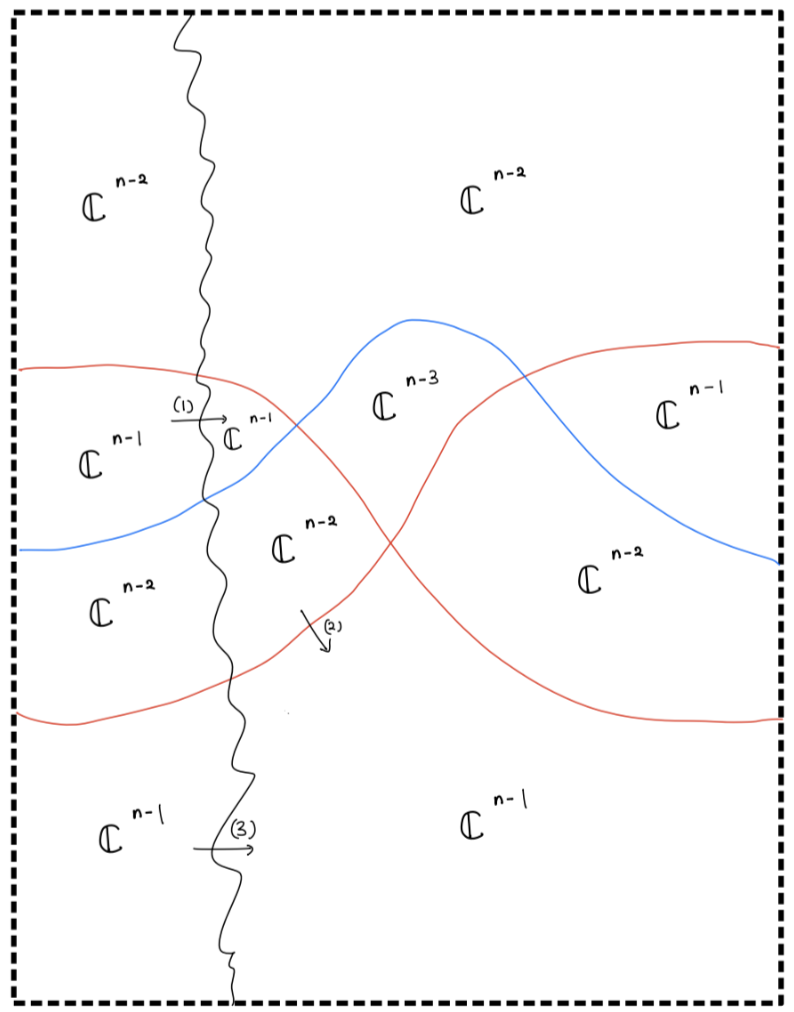
\includegraphics[scale = 0.85]{diagrams/cobord'8/1.png}
    \caption{}
    \label{fig:your-label}
\end{figure}
\textbf{Generizations maps}:
\begin{enumerate}[label = (\arabic*)]
\item $diag(d_n,\cdots,d_2)$
\item $\iota_0 \circ diag(1,\cdots,1) + e'I_{n-1,n-2}$
\item $diag(d_{n-1},\cdots,d_1) + eI_{n-1,n-2}$
\end{enumerate}
where $e' = d_2^{-1}e$. Then we define a cobordism starting from the above sheaf, say $cobord'_8$ supported on $U$. At the end of the cobordism, the sheaf, under the same chart $f$, is described as the following squiggly legible diagram. 
\begin{figure}[H]
    \centering
    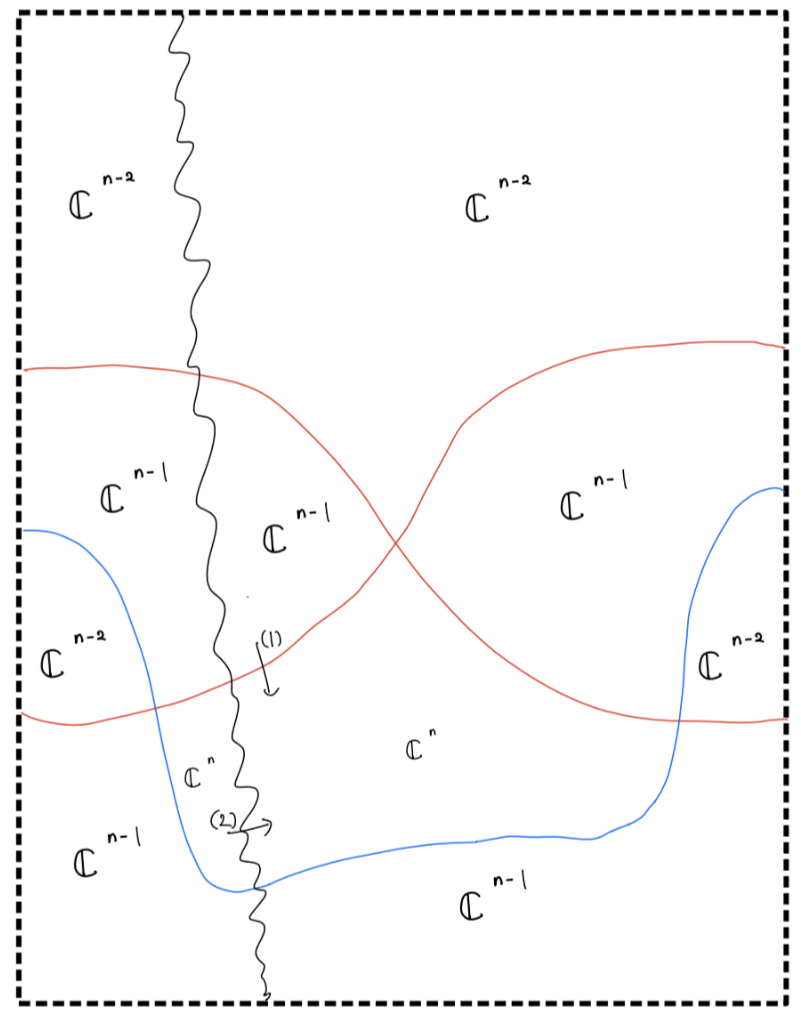
\includegraphics[scale = 0.85]{diagrams/cobord'8/10.png}
    \caption{}
    \label{fig:your-label}
\end{figure}
\textbf{Generizations maps}:
\begin{enumerate}[label = (\arabic*)]
\item $\iota_0 \circ diag(1,\cdots,1) + e'I_{n,n-1}$
\item $diag(d_{n},\cdots,d_1) + eI_{n,n-1}$
\end{enumerate}
\pagebreak
We define $cobord'_8$ as follows.
\begin{enumerate}[label=(Step \arabic*)]
\item we apply $cobord_1$ to the square regions surrounded by purple dotted lines.

\begin{figure}[H]
    \centering
    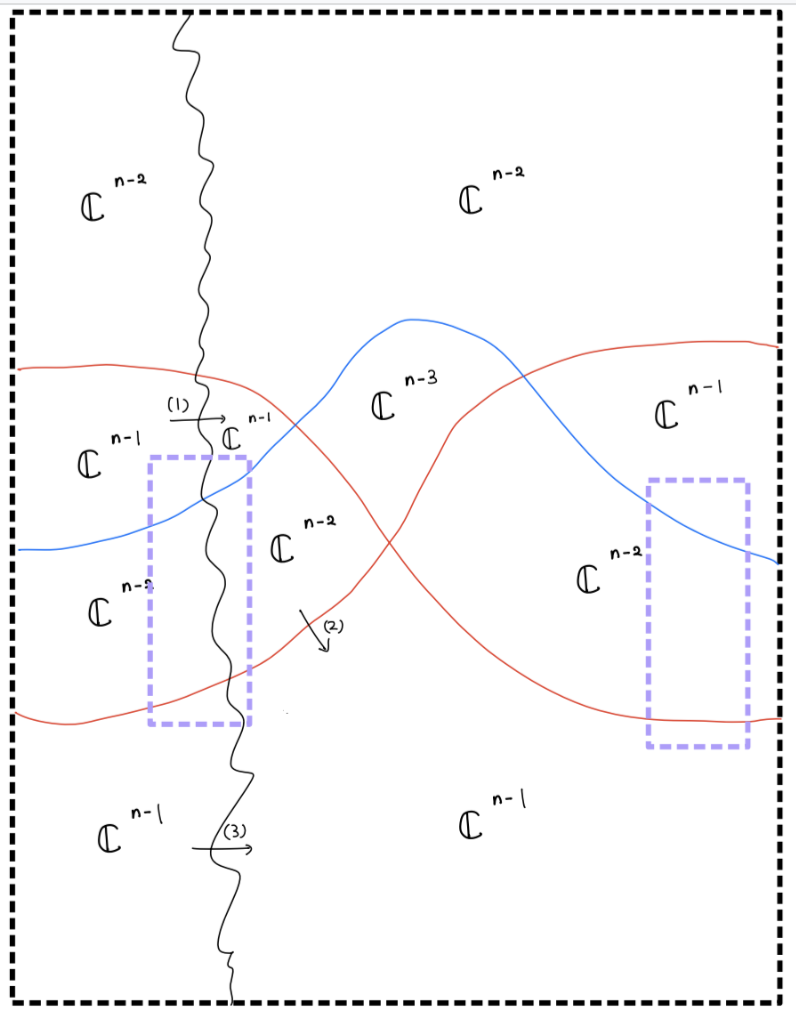
\includegraphics[scale = 0.85]{diagrams/cobord'8/2.png}
    \caption{}
    \label{fig:your-label}
\end{figure}
\pagebreak
we get

\begin{figure}[H]
    \centering
    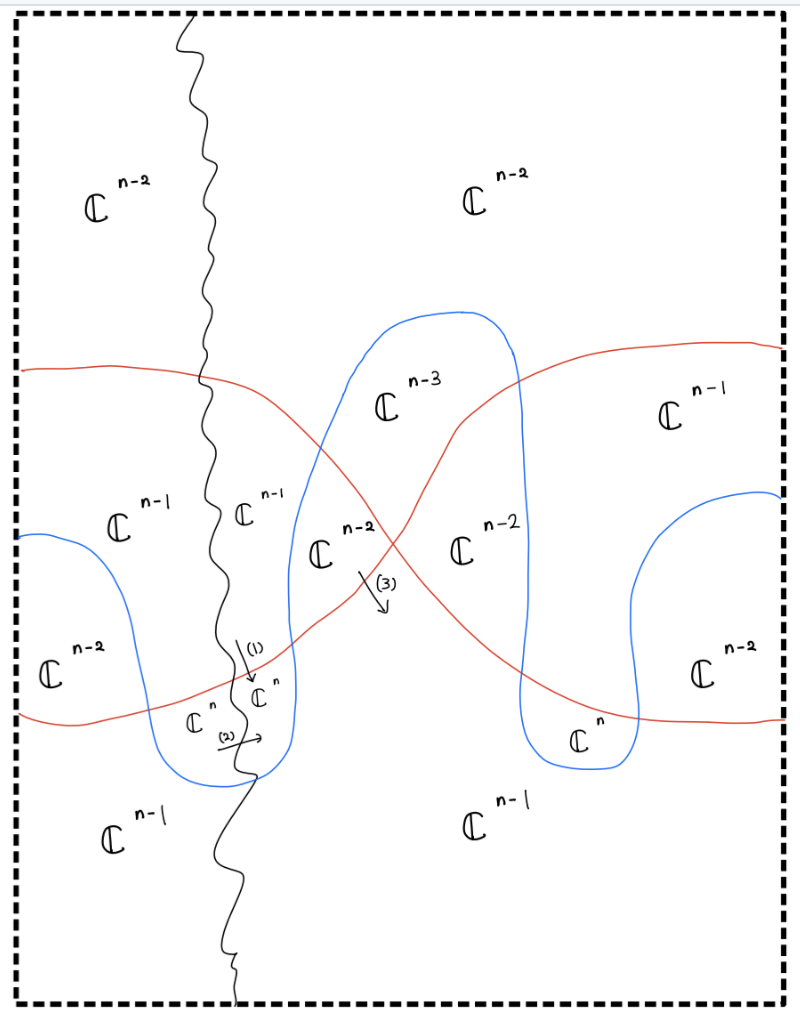
\includegraphics[scale = 0.85]{diagrams/cobord'8/3.png}
    \caption{}
    \label{fig:your-label}
\end{figure}
\textbf{Generizations maps}:
\begin{enumerate}[label = (\arabic*)]
\item $\iota_0 \circ diag(1,\cdots,1) + e'I_{n,n-1}$
\item $diag(d_{n},\cdots,d_1) + eI_{n,n-1}$
\item $\iota_0 \circ diag(1,\cdots,1) + e'I_{n-1,n-2}$
\end{enumerate}
\pagebreak
\item apply $cobord'_4$ to the region surrounded by a purple dotted line.

\begin{figure}[H]
    \centering
    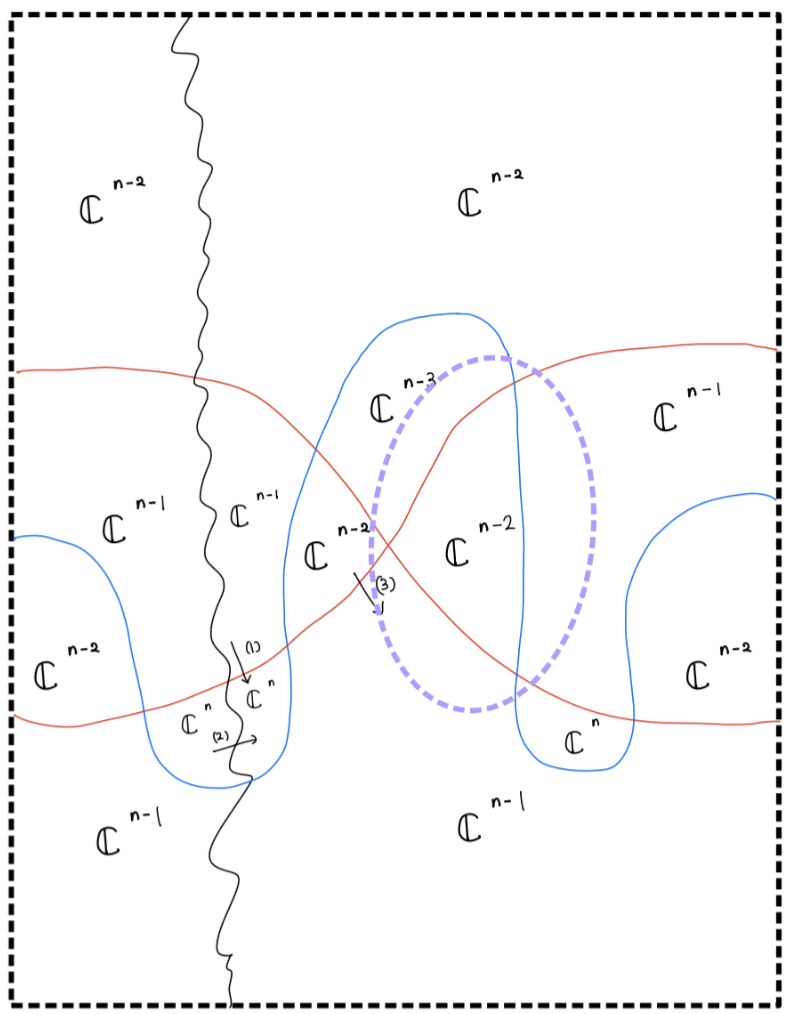
\includegraphics[scale = 0.85]{diagrams/cobord'8/4.png}
    \caption{}
    \label{fig:your-label}
\end{figure}
\pagebreak
we get

\begin{figure}[H]
    \centering
    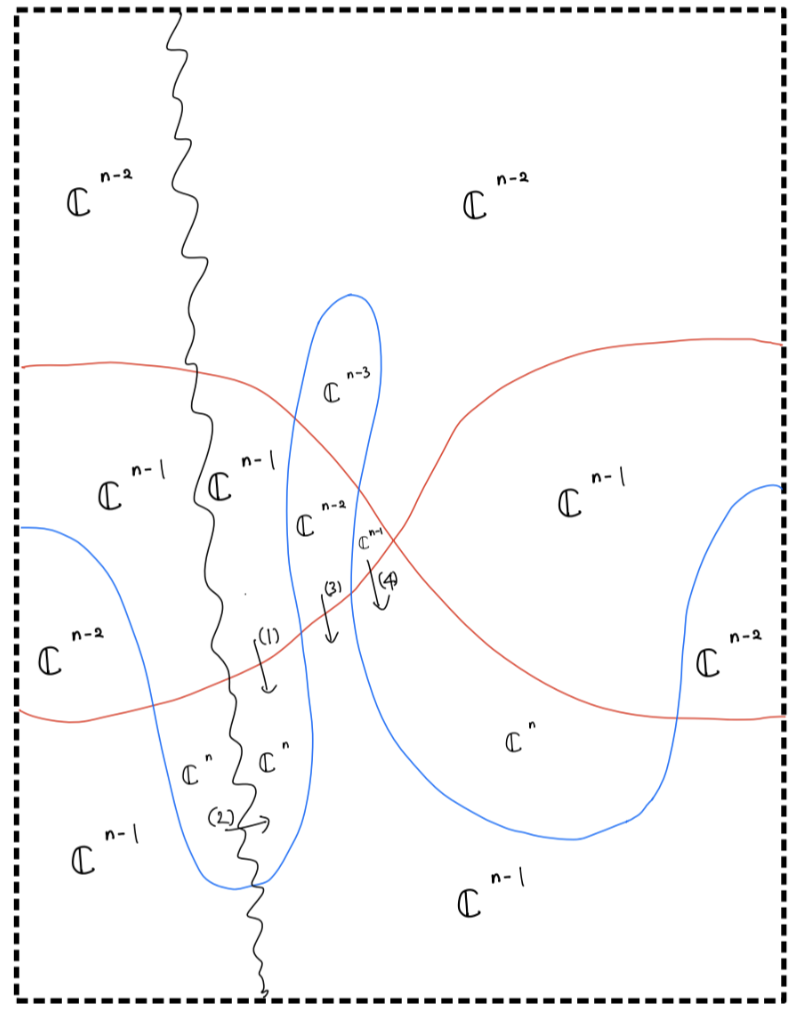
\includegraphics[scale = 0.85]{diagrams/cobord'8/5.png}
    \caption{}
    \label{fig:your-label}
\end{figure}
\textbf{Generizations maps}:
\begin{enumerate}[label = (\arabic*)]
\item $\iota_0 \circ diag(1,\cdots,1) + e'I_{n,n-1}$
\item $diag(d_{n},\cdots,d_1) + eI_{n,n-1}$
\item $\iota_0 \circ diag(1,\cdots,1) + e'I_{n-1,n-2}$
\item $\iota_0 \circ diag(1,\cdots,1) + e'I_{n,n-1}$
\end{enumerate}
\pagebreak
\item apply $cobord_3$ to the region surrounded by a purple dotted line.

\begin{figure}[H]
    \centering
    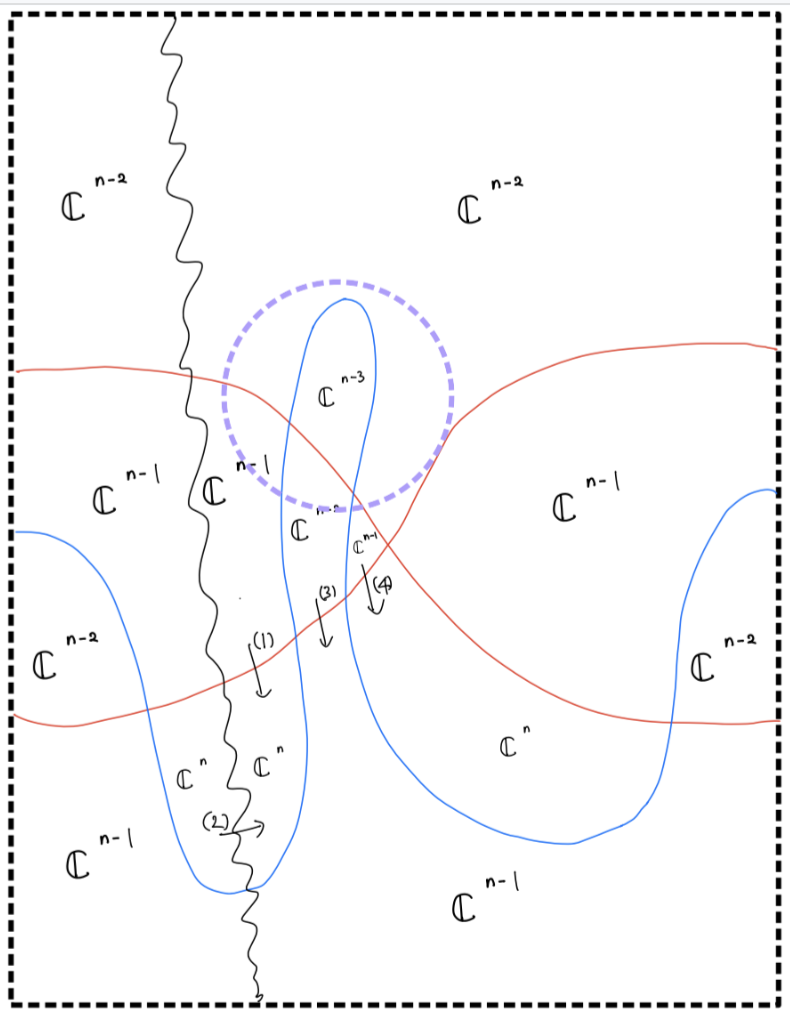
\includegraphics[scale = 0.85]{diagrams/cobord'8/6.png}
    \caption{}
    \label{fig:your-label}
\end{figure}
\pagebreak
we get

\begin{figure}[H]
    \centering
    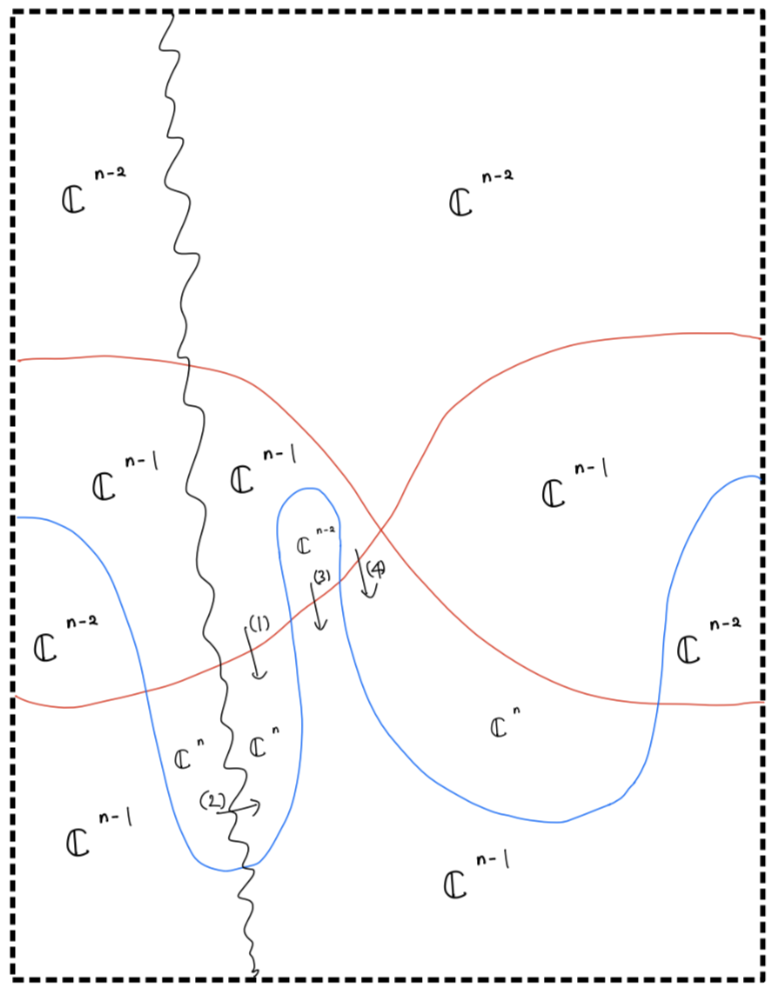
\includegraphics[scale = 0.85]{diagrams/cobord'8/7.png}
    \caption{}
    \label{fig:your-label}
\end{figure}
\textbf{Generizations maps}:
\begin{enumerate}[label = (\arabic*)]
\item $\iota_0 \circ diag(1,\cdots,1) + e'I_{n,n-1}$
\item $diag(d_{n},\cdots,d_1) + eI_{n,n-1}$
\item $\iota_0 \circ diag(1,\cdots,1) + e'I_{n-1,n-2}$
\item $\iota_0 \circ diag(1,\cdots,1) + e'I_{n,n-1}$
\end{enumerate}
\pagebreak
\item apply $cobord_3$ to the region surrounded by a purple dotted line

\begin{figure}[H]
    \centering
    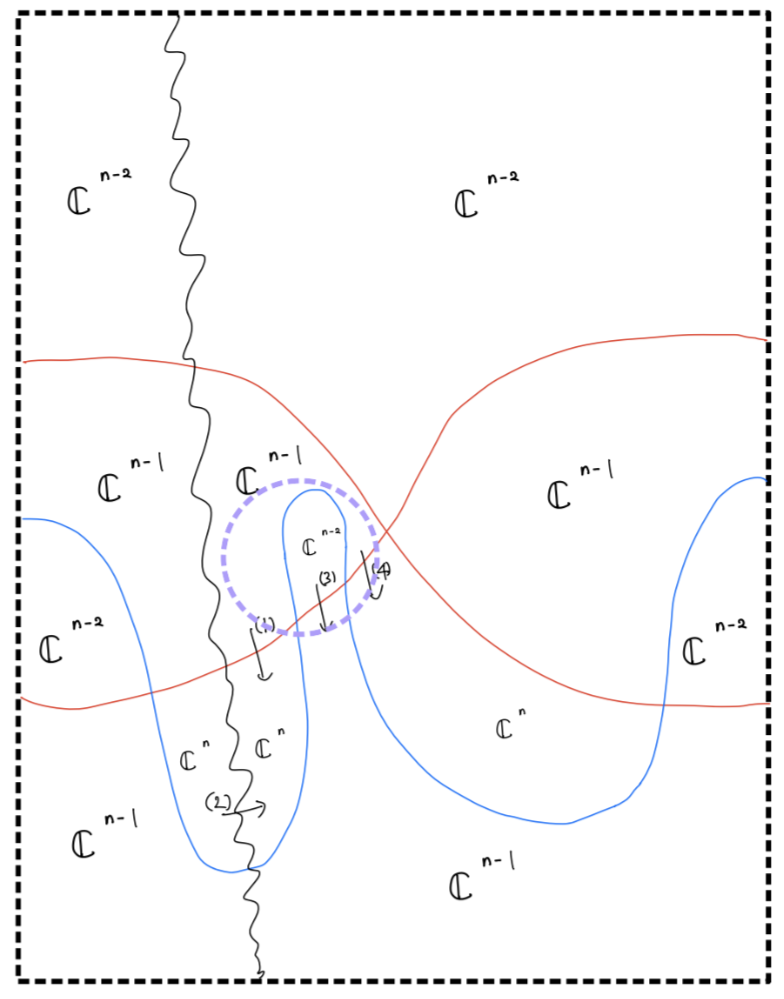
\includegraphics[scale = 0.85]{diagrams/cobord'8/8.png}
    \caption{}
    \label{fig:your-label}
\end{figure}
\pagebreak
we get the final sheaf

\begin{figure}[H]
    \centering
    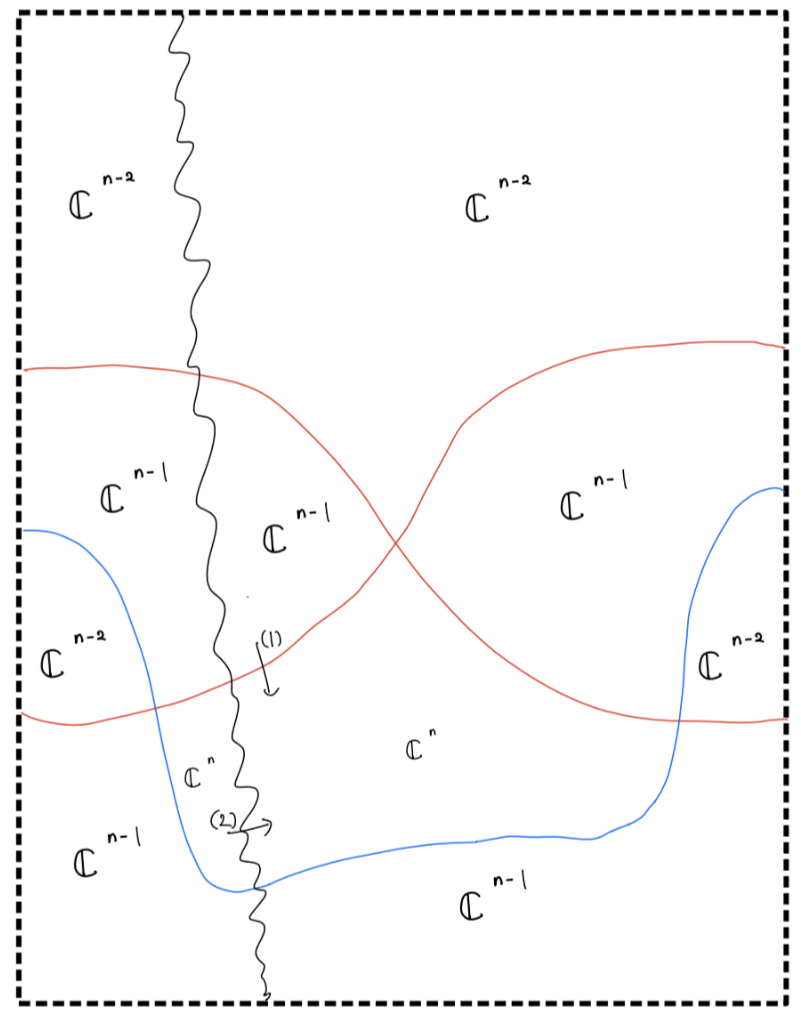
\includegraphics[scale = 0.85]{diagrams/cobord'8/10.png}
    \caption{}
    \label{fig:your-label}
\end{figure}
\textbf{Generizations maps}:
\begin{enumerate}[label = (\arabic*)]
\item $\iota_0 \circ diag(1,\cdots,1) + e'I_{n,n-1}$
\item $diag(d_{n},\cdots,d_1) + eI_{n,n-1}$
\end{enumerate}
\end{enumerate}
\pagebreak